 \pstart \textso{Experim. VIII.} \edtext{Venio}{\lemma{\textso{Experim. VIII.}}\Afootnote{ \textit{ (1) }\ Sumatur \textit{ (2) }\ Venio \textit{ L}}} ad Experimentum quod ego \edtext{in toto}{\lemma{ego}\Afootnote{ \textit{ (1) }\ ad usum philo \textit{ (2) }\ in toto \textit{ L}}} hoc argumento maximi momenti esse judico ad detegendas intimas rerum rationes, etsi sit simplissimum. Nullo hactenus Experimento dijudicari potuit, an aer resistat tantum compressioni\protect\index{Sachverzeichnis}{compressio}, \edtext{tensioni\protect\index{Sachverzeichnis}{tensio} non nisi quatenus alibi tantundem comprimitur;}{\lemma{}\Afootnote{tensioni [...] comprimitur; \textit{ erg.} \textit{ L}}} an \edtext{potius}{\lemma{}\Afootnote{potius \textit{ erg.} \textit{ L}}} resistat tantum tensioni\protect\index{Sachverzeichnis}{tensio} \edtext{seu dilatationi}{\lemma{}\Afootnote{seu dilatationi \textit{ erg.} \textit{ L}}} compressioni\protect\index{Sachverzeichnis}{compressio} vero, non nisi quatenus alibi tantundem tenditur. An vero resistat neque compressioni, neque tensioni\protect\index{Sachverzeichnis}{tensio}, sed generaliter difformitati ut scilicet amet omnia esse aeque tensa, aut omnia esse aeque compressa. Haec quaestio inter primarias habenda est non hujus argumenti tantum, sed et totius philosophiae, cum potissimis naturae phaenomenis aeris compressio\protect\index{Sachverzeichnis}{compressio} tensiove\protect\index{Sachverzeichnis}{tensio} misceatur.
[110 v\textsuperscript{o}] Frustra\edtext{}{\lemma{}\Afootnote{Frustra  \textbar\ innumera \textit{ gestr.}\ \textbar\ machinamenta \textit{ L}}} machinamenta \edtext{quaesivi quibus}{\lemma{machinamenta}\Afootnote{ \textit{ (1) }\ quaesivi ad efficiendum ut aliquod comprimatur in quibus solius vel compressionis\protect\index{Sachverzeichnis}{compressio|textit} vel tensionis\protect\index{Sachverzeichnis}{tensio|textit} \textit{ (2) }\ quaesivi quibus \textit{ L}}} ostenderetur Tensionem\protect\index{Sachverzeichnis}{tensio} \edtext{ solam}{\lemma{Tensionem}\Afootnote{ \textit{ (1) }\ per se \textit{ (2) }\  solam \textit{ L}}}, vel compressionem\protect\index{Sachverzeichnis}{compressio} solam nihil agere, aut totam agere. Nam in experimento 1. ostendi quidem \edtext{sola aeris externi pressione suspendi Mercurium}{\lemma{quidem}\Afootnote{ \textit{ (1) }\ funiculum\protect\index{Sachverzeichnis}{funiculus|textit} a \textit{ (2) }\ sola aeris   \textbar\ externi \textit{ erg.}\ \textbar\  pressione suspendi Mercurium \textit{ L}}}, \edtext{tensione licet}{\lemma{Mercurium,}\Afootnote{ \textit{ (1) }\ pressione licet \textit{ (2) }\ tensione licet \textit{ L}}} aeris \edtext{interni}{\lemma{aeris}\Afootnote{ \textit{ (1) }\ ejus \textit{ (2) }\ interni \textit{ L}}} ablata. Sed nullum experimentum reperire potui quo ostenderem an non fortasse similiter pressione aeris\protect\index{Sachverzeichnis}{pressio!aeris} externi sublata, solaque tensione\protect\index{Sachverzeichnis}{tensio} interni remanente effectus fieret: ac proinde \edtext{an}{\lemma{}\Afootnote{an \textit{ erg.} \textit{ L}}} proprie nec tensioni\protect\index{Sachverzeichnis}{tensio} nec compressioni\protect\index{Sachverzeichnis}{compressio}, sed utrique simul, seu ipsi difformitati ascribendus sit effectus, \edtext{quam}{\lemma{effectus,}\Afootnote{ \textit{ (1) }\ cui scilicet \textit{ (2) }\ quam \textit{ L}}} natura non nisi coacta admittat in Mundo\protect\index{Sachverzeichnis}{mundus}. Nullum inquam, nam etsi in Recipiente Exhausto, pressione aeris\protect\index{Sachverzeichnis}{pressio!aeris} extra Tubum ablata Mercurius\protect\index{Sachverzeichnis}{mercurius} descendat, modo scilicet aere purgatus sit, \edtext{ad hoc tamen responderi potest,}{\lemma{sit,}\Afootnote{ \textit{ (1) }\ id tamen fieri putandum est, \textit{ (2) }\ ad hoc tamen responderi potest, \textit{ L}}} eum a tensione\protect\index{Sachverzeichnis}{tensio} aeris extra Tubum, quippe summe dilatati, et se contrahere conantis fortius trahi, quam a tensione\protect\index{Sachverzeichnis}{tensio} aeris spatium in Tubo relictum implentis. Cum ergo post multam inquisitionem de Experimento ad quaestionem tam profundam resolvendam apto desperarem, ecce occasione Instrumenti inclinationum\protect\index{Sachverzeichnis}{instrumentum!inclinationum} quod longe quaesieram, prope positum inveni. Esto Tubus qualis (instrumenti inclinationi\protect\index{Sachverzeichnis}{instrumentum!inclinationum}) \textit{AB}.  %\begin{wrapfigure}{l}{0.15\textwidth}                    
             %  \begin{center}
                %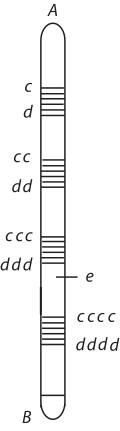
\includegraphics[width=0.15\textwidth]{images/37_3_110v}\\\textit{[Fig. 12]}
                        %\caption{Bildbeschreibung}
                     %   \end{wrapfigure}
                    %    \end{center}
                    %verschoben in 111r
                        %@ @ @ Dies ist eine Abstandszeile - fuer den Fall, dass mehrere figures hintereinander kommen, ohne dass dazwischen laengerer Text steht. Dies kann zu einer Fahlermeldung fuehren. @ @ @ \\
                    In eo ita locetur Mercurius\protect\index{Sachverzeichnis}{mercurius} ut neutrum extremum neque \textit{A} neque \textit{B} attingat \edtext{v. g. in \textit{cd} distantia ab \textit{A} seu linea \textit{Ac} unius pedis, distantia a \textit{B} seu linea \textit{dB} quatuor pedum assumta}{\lemma{v. g.}\Afootnote{in [...] a \textit{B}   \textbar\ seu linea \textit{dB} \textit{ erg.}\ \textbar\  quatuor pedum assumta \textit{ erg.} \textit{ L}}}. Hoc facto Tubus claudatur, \edtext{quod ope Epistomii\protect\index{Sachverzeichnis}{epistomium} alicujus circumacti facile fieri potest}{\lemma{}\Afootnote{quod [...] potest \textit{ erg.} \textit{ L}}}. Intelligatur primum aer in Tubo esse ordinarius, seu neque tensus neque compressus, modo scilicet Tubus sit Horizontalis. Hoc facto Tubus erigatur in situm perpendicularem \textit{A} sursum \textit{d} deorsum spectante, noteturque in quantam altitudinem Mercurius\protect\index{Sachverzeichnis}{mercurius} pondere suo descendat ita enim necessario intelligitur quantum comprimat aerem sub se, seu inter se et \textit{B} et quantum tendat aerem supra se seu inter se et \textit{A}. \edtext{Ponatur}{\lemma{\textit{A}.}\Afootnote{ \textit{ (1) }\ Hoc facto Tubus iterum aperiatur \textit{ (2) }\ Ponatur \textit{ L}}} delabi per altitudinem pedis seu \edtext{ex \textit{cd}}{\lemma{}\Afootnote{ex \textit{cd} \textit{ erg.} \textit{ L}}} in \textit{cc-dd} manifestum est aerem \edtext{superiorem}{\lemma{superiorem}\Afootnote{\textit{ erg.} \textit{ L}}} in \textit{Ac} \edtext{spatio unius pedis initio comprehensum,}{\lemma{\textit{Ac}}\Afootnote{ \textit{ (1) }\ initio comprehensum, unius \textit{ (2) }\ spatio unius pedis initio comprehensum, \textit{ L}}} nunc implere debere spatium \textit{A-cc} pedum duorum, ac proinde esse duplo \edtext{dilatatiorem}{\lemma{duplo}\Afootnote{ \textit{ (1) }\ tensionem\protect\index{Sachverzeichnis}{tensio|textit} \textit{ (2) }\ dilatatiorem \textit{ L}}}.\footnote{\textit{In der rechten Spalte:} NB. Nova immittenda.   
                 %   \textbar\ NB. Baroscopium\protect\index{Sachverzeichnis}{baroscopium} in quo Embolus\protect\index{Sachverzeichnis}{embolus} Elaterio\protect\index{Sachverzeichnis}{elaterium} moveatur etiam sursum invita aeris gravitate\protect\index{Sachverzeichnis}{gravitas!aeris}. \textit{ erg.}\ \textbar\ 
                NB. Baroscopium\protect\index{Sachverzeichnis}{baroscopium} in quo Embolus\protect\index{Sachverzeichnis}{embolus} Elaterio\protect\index{Sachverzeichnis}{elaterium} moveatur etiam sursum invita aeris gravitate\protect\index{Sachverzeichnis}{gravitas!aeris}.
                     Experiendum in diversis gradibus. Experiendum in Camera clausa seu vase clauso exiguo. An 
                 %     \textbar\ notabilis \textit{ gestr.}\ \textbar\ 
                      differentia altitudinis in aere libero? Hinc differentia inter liberum et clausum in aere libero inseratur summo Tubo aer diversae magnitudinis ad explorandam diversitatem detrahendo aperiat continue foramen Mercurii\protect\index{Sachverzeichnis}{mercurius} aut detrahat vesicam Embolumque\protect\index{Sachverzeichnis}{embolus} videndum an fatigetur  descensus quia tensio\protect\index{Sachverzeichnis}{tensio} nulla. Addatur longitudini totius tubi, posita tensione\protect\index{Sachverzeichnis}{tensio} falsum semper descendere ad idem punctum. An in ipso aere externo funiculus\protect\index{Sachverzeichnis}{funiculus} seu tensio\protect\index{Sachverzeichnis}{tensio}. }
                    Contra aerem \edtext{inferiorem}{\lemma{inferiorem}\Afootnote{\textbar\ qui \textit{ gestr.}\ \textbar\ in \textit{ L}}} in \textit{dB} spatio quatuor pedum initio comprehensum, nunc comprehendi tantum spatio \textit{dd-B} pedum trium. Est ergo tensio\protect\index{Sachverzeichnis}{tensio} \edtext{ante descensum ad tensionem post descensum}{\lemma{tensio}\Afootnote{ \textit{ (1) }\ prior ad posteriorem \textit{ (2) }\ ante [...] descensum \textit{ L}}} ut 1. ad 2. compressio\protect\index{Sachverzeichnis}{compressio} \edtext{illa ad hanc}{\lemma{compressio}\Afootnote{ \textit{ (1) }\ prior ad posteriorem \textit{ (2) }\ illa ad hanc \textit{ L}}}, ut 3. ad 4. His ita notatis aperiatur Tubus \textit{AB} utrinque, et sublata ita omni compressione\protect\index{Sachverzeichnis}{compressio} ac tensione\protect\index{Sachverzeichnis}{tensio}, aereque in statum ordinarium remisso, Mercurius\protect\index{Sachverzeichnis}{mercurius} ponatur in loco \textit{cc-dd} (cum antea positus fuerit in loco \textit{cd}). Tubus iterum utrinque claudatur \edtext{erigaturque: altitudo}{\lemma{erigaturque:}\Afootnote{ \textit{ (1) }\ Eventus et \textit{ (2) }\ altitudo \textit{ L}}} %
                    %Afootnotes zur footnote
\edtext{}{\lemma{NB.}\linenum{|11|||12|}\Afootnote{Baroscopium\protect\index{Sachverzeichnis}{baroscopium}\protect\index{Sachverzeichnis}{baroscopium|see{barom\'{e}tre u. barometrum}} in quo Embolus\protect\index{Sachverzeichnis}{embolus} Elaterio\protect\index{Sachverzeichnis}{elaterium} moveatur etiam sursum invita aeris gravitate\protect\index{Sachverzeichnis}{gravitas!aeris}. \textit{ erg. L}\hspace{20pt} 13f.\hspace{6pt} An\ \textbar\ notabilis \textit{ gestr.}\ \textbar\ differentia \textit{L}}}%{\lemma{An}\linenum{|13|||13|}\Afootnote{ \textbar\ notabilis \textit{ gestr.}\ \textbar\ differentia}}
%\edtext{}{\lemma{An}\linenum{|13|||13|}\Afootnote{ \textbar\ notabilis \textit{ gestr.}\ \textbar\ differentia}}
                                         descensus futura quaestionem nostram infallibili demonstratione \edtext{terminabit.}{\lemma{demonstratione}\Afootnote{ \textit{ (1) }\ determinabit \textit{ (2) }\ terminabit. \textit{ L}}} \edtext{Compressio ante descensum sit ad compressionem post descensum ut 3. ad 4.}{\lemma{terminabit.}\Afootnote{ \textit{ (1) }\ Nam si  \textit{(a)}\ tensio\protect\index{Sachverzeichnis}{tensio|textit} \textit{(b)}\ sola compressio  \textit{(aa)}\ violenta est \textit{(bb)}\ aeri   \textbar\ per se \textit{ erg.}\ \textbar\  violenta est, tensio\protect\index{Sachverzeichnis}{tensio|textit} vero non nisi per accidens quatenus sequitur compressionem, sequitur eandem fore compressionem nunc, quam ante, eadem enim est vis premens, ac proinde aer in spatio \textit{dd-B} trium pedum, redigetur in spatium $\displaystyle\frac{9}{4}$ pedum  \textit{(aaa)}\ quod est ad prius \textit{(bbb)}\ seu compressio, (quae est in reciproca spatiorum ratione)  \textit{(aaaa)}\ erit ut ante ad priorem seu statum natura \textit{(bbbb)}\ erit quemadmodum ante; ut scilicet status ante sint ut 4 ad 3. \textit{ (2) }\  Compressio  \textit{(a)}\ prior ad posteriorem \textit{(b)}\ ante [...] 4. \textit{ L}}} Quia spatia 
                                         [111 r\textsuperscript{o}] sunt ut 4. ad 3. Nulla tensionis\protect\index{Sachverzeichnis}{tensio} ratione habita seu etsi priori non concordet, ante enim ex uno pede fiebant duo, nunc ex duobus pedibus supra Mercurium\protect\index{Sachverzeichnis}{mercurius} fiunt $\rule[-4mm]{0mm}{10mm}\displaystyle\frac{11}{4}$. Tota enim tubi \edtext{capacitas (demto loco a Mercurio repleto) est}{\lemma{tubi}\Afootnote{ \textit{ (1) }\ vacuitas est \textit{ (2) }\ capacitas [...] est \textit{ L}}} 5 pedum seu $\rule[-4mm]{0mm}{10mm}\displaystyle\frac{20}{4}$ a quibus demtis $\rule[-4mm]{0mm}{10mm}\displaystyle\frac{9}{4}$. manent $\rule[-4mm]{0mm}{10mm}\displaystyle\frac{11}{4}$. delabetur ergo Mercurius\protect\index{Sachverzeichnis}{mercurius} ex \textit{cc-dd} in \textit{ccc-ddd} ita ut spatium \textit{ddd-B} sit $\rule[-4mm]{0mm}{10mm}\displaystyle\frac{9}{4}$. \textit{A-ccc} sit $\rule[-4mm]{0mm}{10mm}\displaystyle\frac{11}{4}$.
                                         \pend